% Why the deltas of two disjoint swaps do not add up: the m x n grid of operations,
% two swaps S1 (columns 2,3) and S2 (columns 6,7), the join between columns c and c+1,
% and two lattice paths that cross the join in different rows.
\documentclass[tikz,border=2pt]{standalone}
\usepackage{amsmath}
\usetikzlibrary{arrows.meta}
\begin{document}
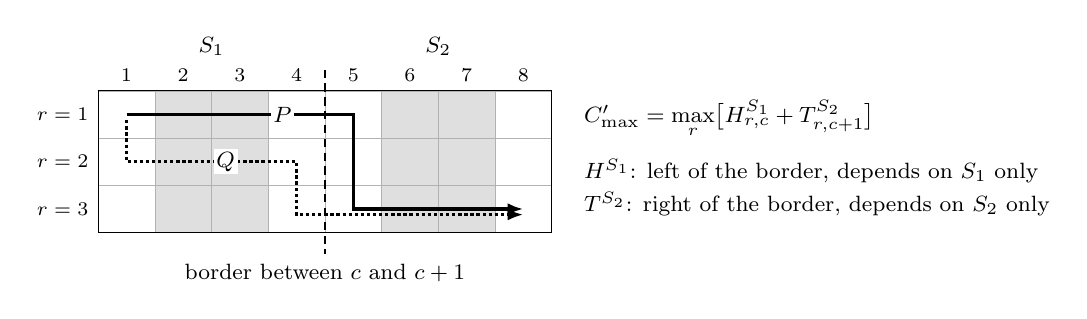
\begin{tikzpicture}[x=0.72cm,y=0.6cm,font=\footnotesize]
% swapped columns
\foreach \c in {2,3}{\fill[gray!25] (\c-1,0) rectangle (\c,-3);}
\foreach \c in {6,7}{\fill[gray!25] (\c-1,0) rectangle (\c,-3);}
% grid
\foreach \c in {0,...,8}{\draw[gray!60,very thin] (\c,0) -- (\c,-3);}
\foreach \r in {0,...,3}{\draw[gray!60,very thin] (0,-\r) -- (8,-\r);}
\draw (0,0) rectangle (8,-3);
\foreach \c in {1,...,8}{\node[above] at (\c-0.5,0) {\scriptsize\c};}
\foreach \r in {1,...,3}{\node[left] at (0,-\r+0.5) {\scriptsize $r=\r$};}
\node[above] at (2,0.55) {$S_1$};
\node[above] at (6,0.55) {$S_2$};
% join
\draw[thick,densely dashed] (4,0.45) -- (4,-3.45);
\node[below,align=center] at (4,-3.45) {border between $c$ and $c+1$};
% path P (solid): row 1 to column 5, then down to row 3
\draw[very thick,-{Latex[length=2mm]}] (0.5,-0.5) -- (4.5,-0.5) -- (4.5,-2.5) -- (7.5,-2.5);
\node[fill=white,inner sep=1pt] at (3.25,-0.5) {$P$};
% path Q (dashed): down at column 1, row 3 to the end
\draw[very thick,densely dotted,-{Latex[length=2mm]}] (0.5,-0.62) -- (0.5,-1.5) -- (3.5,-1.5) -- (3.5,-2.62) -- (7.5,-2.62);
\node[fill=white,inner sep=1pt] at (2.25,-1.5) {$Q$};
% head / tail labels
\node[anchor=west] at (8.4,-0.6) {$C'_{\max}=\max\limits_{r}\bigl[H^{S_1}_{r,c}+T^{S_2}_{r,c+1}\bigr]$};
\node[anchor=west] at (8.4,-1.7) {$H^{S_1}$: left of the border, depends on $S_1$ only};
\node[anchor=west] at (8.4,-2.4) {$T^{S_2}$: right of the border, depends on $S_2$ only};
\end{tikzpicture}
\end{document}
